\documentclass{cmn}

\begin{document}
  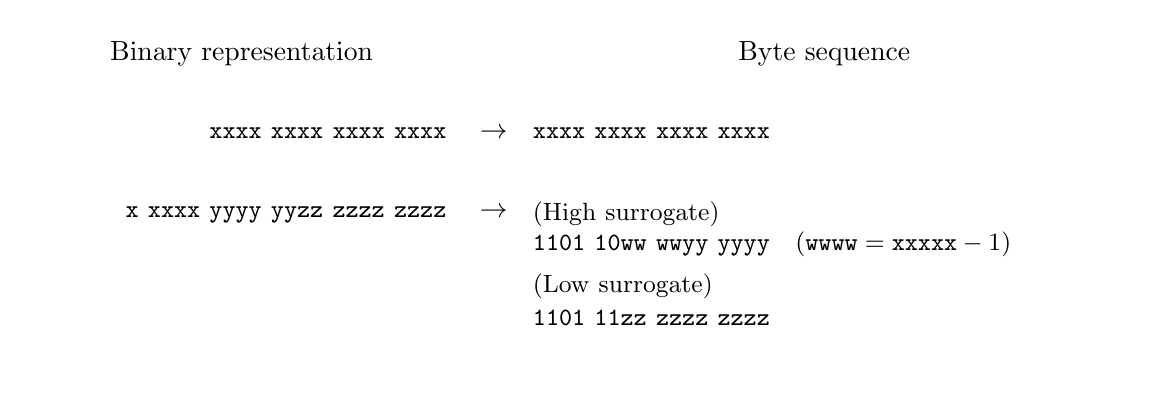
\begin{tikzpicture}
    \node[text width=52mm,align=center] at (0,0) {Binary representation\strut};
    \node[text width=52mm,align=right] at (0,-10mm) {\small\texttt{xxxx xxxx xxxx xxxx}\strut};
    \node[text width=52mm,align=right] at (0,-20mm) {\small\texttt{x xxxx yyyy yyzz zzzz zzzz}\strut};

    \node at (32mm,-10mm) {$\rightarrow$\strut};
    \node at (32mm,-20mm) {$\rightarrow$\strut};

    \node[text width=74mm,align=center] at (74mm,0) {Byte sequence};
    \node[text width=74mm,align=left] at (74mm,-10mm) {\small\texttt{xxxx xxxx xxxx xxxx}\strut};
    \node[text width=74mm,align=left,text depth=0mm,minimum height=42.5mm] at (74mm,-20mm) {\small (High surrogate)\\
      \texttt{1101 10ww wwyy yyyy}\strut \quad$(\texttt{wwww} = \texttt{xxxxx}-1)$\\
      \vspace{4pt}
      (Low surrogate) \\
      \texttt{1101 11zz zzzz zzzz}\strut};
  \end{tikzpicture}
\end{document}
